\documentclass[]{article}

\usepackage[utf8]{inputenc}
\usepackage[paperheight=0.6in,paperwidth=1.7in,margin=.1mm]{geometry}
\usepackage{tikz}
\usetikzlibrary{shapes, arrows, calc}
\usepackage{color}

\usepackage{booktabs}  % nicer table borders 

\begin{document}

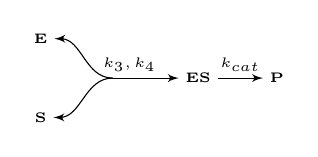
\begin{tikzpicture}[>=latex']
\tiny
\node  at (0, 0)   (E) {$\bf E$};
\node  at (0, -1)  (S) {$\bf S$};
\node  at (2, -.5) (ES) {$\bf ES$};
\node  at (1, -.5) (fakeES) {};
\node  at (3, -.5) (P) {$\bf P$};
\path (E) edge[<-, out=0, in=180] (fakeES);
\path (S) edge[<-, out=0, in=180] (fakeES);
\path ($(fakeES)+(-.1,0)$) edge[->] node[above, xshift=-0.2cm] 
    {$k_3, k_4$} (ES);
\path (ES) edge[->, out=0, in=180] node[above] {$k_{cat}$} (P);
\end{tikzpicture} 
\end{document}

